\section{Detailed hardware setup}

The wireless network system consists of a Hub and sensor nodes. After careful examination of all available nodes the Multi-standard SensorTag from Texas instruments \cite{TIsensortag} was chosen. A Crossbow Telos B node has been used as sink for the network and as interface with the Raspberry Pi board. 
Initially, a completely different system was designed. It was made with an XigBee board as a link between the nodes and the Raspberry pi. However, because of lack of documentation of the SensorTags and its actual zigbee protocol support, development with it could not continue. Instead, the highly research and documented TelosB Crowbow node was preferred.


\subsection{Sensor Node - TI Sensor Tag}

The General requirements for the node were design for durability, optimal functionality and user friendly application. This sensor application requires many precise design parameters from the node but those can not all be satisfied. Thus, the general requirements will be discussed and then shown how well the TI sensor tag fulfills them and how it could be added. With the time scope of the project, some of these requirements will not be met, rather a focus will be but on functionality of current components.

In general the nodes have to be small in size to fit even in small plant pots. They should be battery powered and in order to be able to acquire the necessary data, they need to have sensors in and above the soil. Moreover, the nodes should be waterproof, contain a status-LED and a RF-module for wireless communication with the Hub.

Each sensor node should be able to measure the items listed in Table \ref{list-req} and if the sensor tag fulfills them or not.
\begin{table}[htbp]
	\centering
	\begin{tabular}{lc}
		\toprule
		Requirements & \multicolumn{1}{l}{TI sensor tag} \\ 
		\midrule
		Brightness & yes \\ 
		Temperature & yes \\ 
		Soil humidity & no \\ 
		Air humidity & yes \\ 
		Soil Ph-value & no \\
		\bottomrule 
	\end{tabular}
	\vspace{0.1cm}
	\caption{Requirement compared to the capabilities of the TI sensor tag}
	\label{list-req}
\end{table}


A high sampling rate is not necessary and therefore keeping the sampling rate to a minimum increases battery life substantially. For the same reason it is advisable to decrease the transmission rate by only sending data upon significant change.

\subsubsection{Detailed hardware design}

The sensor tag from TI can measure many things which are useful for the project and was chosen were it also offers various connection methods via BLE, Zigbee, 6LowWPAN and soon wifi. Its battery lasts a year with one second report intervals and is easily replaceable be the user. 

The multi-standard processor, CC2560 \cite{block-cc2650}, connects to ten low power MEMS (Microelectromechanical systems) \cite{MEMS} sensors seen in Figure \ref{fig:sensors}. This makes it possible to be extremely small (micrometers), light weight, mobile and robust.

\begin{figure}[!h]
	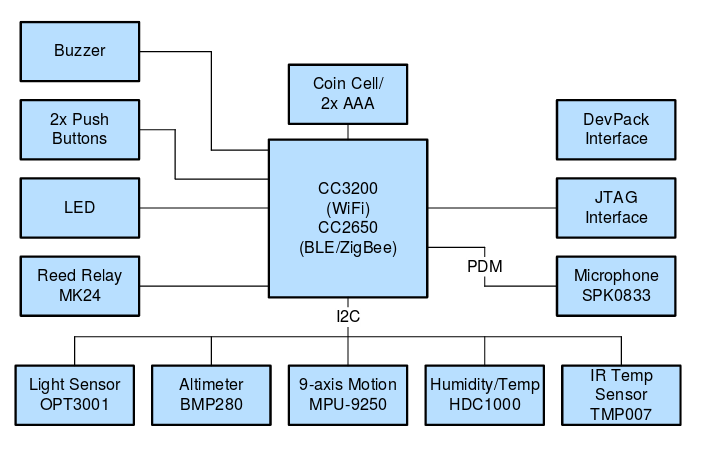
\includegraphics[width=\linewidth]{sensors-layout}
	\caption{Block diagram of the MEMSs sensors and the CC2650 processor \cite{block-cc2650}.}
	\label{fig:sensors}
\end{figure}


\subsection{Hub - Raspberry Pi 3}
The Hub has to be able to collect all data provided from the nodes. It can be connected to the buildings power grid and Internet. A user interface (UI) should be digitally accessible via touchscreen, web page and/or app. Additionally the system should be able to inform the user about critical sensor values. To decide whether a value is critical or not, the Hub has to know which type of plant the sensor monitors and then check a Internet database for specific requirements or rely on user defined values.
The Raspberry pi 3, will be referred to as the Pi, is able to connect to the internet via wifi or ethernet without extra adapters. The Pi used in this application is 3 model b that differ from the previous hardware because the addition of A
802.11n Wireless LAN, the Bluetooth 4.1 and Bluethooth Low Energy (BLE). Furthermore, the processos has been upgraded to a 1.2GHz 64-bit quad-core ARMv8 CPU. \cite{pi}\\

\subsection{Crossbow TelosB}
In this application also another type of node has been used: Crossbow TelosB. It is developed by the University of California, Berkley and it is based on the open source TelosB / Tmote Sky platform. 
The main advantages of this sensor node is the presence of a USB hardware interface for direct communication with the Pi. The node will used as a link between the Raspberry and the sensor network composed of the TI sensortag nodes, see Figure \ref{fig:Architecture}.
The Crossbow TelosB is equipped with a 802.15.4 compliant transceiver, humidity, temperature and light sensor and it is powered by 2 AA batteries. The node is able to run Contiki and TinyOs \cite{TB}.\\

